\documentclass[12pt,a4paper]{article}
\usepackage[utf8]{inputenc}
\usepackage[french]{babel}
\usepackage[T1]{fontenc}
\usepackage{amsmath}
\usepackage{amsfonts}
\usepackage{amssymb}
\usepackage{graphicx}
\usepackage[left=2cm,right=2cm,top=2cm,bottom=2cm]{geometry}
\usepackage[hidelinks]{hyperref}
\usepackage{multirow}
\usepackage{caption}
\usepackage{float} 
 
\usepackage{titlesec}%controler la taille du titre 
\titleformat{\chapter}[display] %titre du chapitre
	{\normalfont\fontsize{30pt}{0}\bfseries}
	{\chaptertitlename\thechapter}{14pt}{}
\titleformat{\section} % controle de section
	{\normalfont\fontsize{14pt}{0}\bfseries}
	{\thesection}{6pt}{} % espace entre le numéro et le titre

\begin{document}

\title{
	{\textbf{{\Huge CAHIER DE CHARGE}}}\\
	\vspace*{2cm}
	{Développement d'un module de signature électronique (PKI)}
}

%\vspace*{3cm}
\author{Oumar Djimé RATOU\\
{\small \href{mailto:oudjira90@yahoo.com}{oudjira90@yahoo.com}}}
 

\maketitle


\newpage
\tableofcontents
\newpage

%**************
\listoffigures
%*************
\newpage
%----------------
\listoftables
%------------------
\newpage
%\begin{flushleft}


\section{Description et compréhension du projet}

	Le projet soumis à mon analyse consiste à mettre sur pied un module de signature électronique (dite \textbf{numérique} est un moyen permettant d'identifier son propriétaire et garantir l'authenticité et l'intégrité du contenu)  basant sur  l'infrastructure à clés publique(ICP) ou la Public key infrastructure (PKI). Il va consister  dans un premier temps :\\
	\begin{itemize}
		\item générer la paire de clés (publiques et privées):
		\item générer un certificat auto-signé.\\
\end{itemize}		
	   Et ensuite :\\
	\begin{itemize}
	\item calculer une valeur de hachage du document(empreinte numérique),
	\item chiffrer l'empreinte générée avec la clé privée,
	\item associer l'empreinte au document,
	\item vérifier la signature avec la clé publique.\\
\end{itemize}		   
	
	 Ainsi le module permettra à d'autres développeurs d'intégrer facilement dans leur plate-forme de même technologie afin que les utilisateurs finaux puissent l'utiliser aisément.\\
	 
	 Ou encore on peut facilement l'importer dans un programme quelconque de même technologie (langage de programmation) et utiliser les fonctionnalités, à l'exemple du module \textbf{math} sous python : on fait juste \textbf{import math} pour utilisé tous les fonctionnalités de la bibliothèque \textbf{math} ou on fait \textbf{from math import sqrt } pour importer seulement la fonction racine carré. Notre module comportera exactement de la même façon.

\section{Étude de la faisabilité technique}
	\subsection{Contexte et problématique} 
	
		La création des signatures électronique basant sur les infrastructures à clé publiques que sa soit avec OpenSSL ou d'autres se font soit en console, soit d'utiliser des outils propriétaires tels que :
		\begin{itemize}
			\item Word pour Microsoft,
			\item Adobe Reader de l'entreprise Adobe,
			\item DocuSign,
			\item Eversign,
			\item Yousign,\\
		\end{itemize}
		
		soit d'aller chez une Autorité de Certification (AC) pour générer un certificat, qui sont complexes et coûteux pour les utilisateurs et surtout à ceux qui débutent en développement des applications et en sécurité informatique. Et encore malheureusement ils sont déjà intégrés dans leurs applications complètes, donc pas des moyens de les réutiliser dans  d'autres logiciels comme des modules.\\
		
		Par ailleurs d'autres ne sont pas dans les systèmes d'exploitation libre(open source) comme Linux, par exemple Word de Microsoft et Adobe Reader ne fonctionnent pas sous Linux. 
		
		\newpage
		
		Les problèmes qui surviennent souvent dans les entreprises en particulier et chez les développeurs en général c'est la disposition des programmes modulaires pour intégrer facilement dans leurs plates-formes en fin de gagner en temps et en l'argent (surtout pour les entreprises). Ces nécessités nous amènent à nous poser les questions suivantes:\\
		
	\begin{itemize}
		\item Comment peut-on rendre cette difficulté de signer un document de manière transparente?
		\item Comment faciliter le développement d'un outil informatique au sein de l'entreprise ?
		
		\item Comment développer un module multi-plateforme ?
	\end{itemize}
	
	
	
	\subsection{Objectifs}
		\subsubsection{Objectif global}
			Il sera question pour moi de développer un module des gestions des signatures basant sur les infrastructures à clé publique et le rendre modulaire.
		\subsubsection{Objectif spécifique}
			De façon spécifique, il sera question pour moi de gérer les problèmes spécifiques liés aux :
			\begin{itemize}
				\item Création d'une signature des documents numériques (texte, son, vidéo, PDF, etc.) en se basant sur les infrastructures à clé publique ou PKI,
				\item automatisation de la création des la signature à la main,
				\item vérification de la signature de document numérique,
				\item prouver l'authenticité d'un signataire,
				\item faciliter à l'entreprise lors d'un besoin d'un module de signature électronique,
			
				\item rendre la vie facile au développeur qui ne maîtrise pas forcément  la notion de cryptographie qui se cache derrière la signature numérique, d'intégrer ce module dans sa plate-forme.\\
				%\item  
			\end{itemize}
			Ainsi les utilisateur avertis pourront juste l'importer dans leurs programmes et l'utilisé facilement. Tout ce qu'un utilisateur doit connaître c'est le nom de la méthode qu'il veut appeler avec sa signature (les paramètres de la méthode) et la méthode retournera le résultat voulu. Il y'aura une commande d'aide si l'utilisateur ne connais pas le nom de la méthode  avec sa signature(paramètre) et une manuelle bien documenté avec des exemples d'utilisations.	
				%\subsection{Les outils nécessaires}
			
	
	%\begin{minipage}{\textwidth}
		\subsubsection*{Environnement}
		
		 
		    L’environnement dans lequel nous nous trouvons est favorable au projet puisqu’un
tel système existe certes mais sous une licence payante  et non modulable. Sa mise en œuvre sera une innovation importante dans l’évolution numérique au sein de l'entreprise.
	%\end{minipage}
\newpage
\section{Description des besoins}

	\subsection{Spécifications fonctionnelles}
	
	Notre module de signature électronique aura comme spécification fonctionnelle :
	
	\begin{itemize}
		\item générer des paires de clés(publique et privée) ,
		\item générer un certificat (auto-signé, puisque le signé est payant)
		\item signer un document numérique à l'aide de la clé privée,
		\item vérifier la signature d'un document numérique à l'aide de la clé publique,
		\item chiffrer/déchiffrer un document,
		\item générer un Hash d'un document.\\
	\end{itemize}
	
	\textbf{Explication de chaque fonctionnalité : } au préalable on import d'abord le module dans notre programme:\\
	
		\begin{enumerate}
			\item pour générer une paire de clé rien de plus compliqué on suppose que le nom de la fonction s'appelle genererPaireKey(algo, taille) et prend en paramètre l'algorithme (RSA par exemple) et la taille de clé (2048 bits par exemple), la commande finale sera \textbf{ genererPaireKey(RSA, 2048)}, ainsi la méthode nous retournera une paire de clé RSA de taille 2048 bits (ex. OpenSSL). On pourra aller plus loin en protégeant la clé avec un algorithme symétrique, ça veut dire que les paramètres augmenteront et deviendra\textbf{ genererPaireKey(algoAsym, algoSym, taille)} dont la commande finale sera \textbf{genererPaireKey(RSA, 3DES, 2048)}, du coup après la validation on demandera d'entré un mot de passe deux fois de suite. Ainsi on se retrouvera avec un système complet et sécurisé.
			
			\item la génération du certificat par une autorité de certification(AC) doit respecter la spécification de la norme x.509, on aura les paramètres obligatoires suivants:
			\begin{itemize}
				\item Country Name (ex. CM),
				\item Locality Name (ex. YAOUNDÉ),
				\item Organizational Unit Name (ex. ITS ),
				\item Common Name (ex. CRYPTO),
				\item  Email Address (ex. its@gmail.com)
			\end{itemize}
			
			\item la signature d'un document à besoin de plusieurs paramètres(fichier ou document ,clé privée et clé publique ,certificat, le Hash du fichier ) dans deux scénarios:\\
		
			
			\textbf{Expéditeur : Signature}	\\
			\begin{itemize}
				\item Condensation du contenu : on hache le fichier avec une fonction de hachage (ex. SHA256) et on obtiendra un condensé de 63 bits quelque soit la taille du document,
				\item On crypte le résultat précédente avec un algorithme asymétrique en utilisant la clé secrète,
				\item En suite on associe un certificat délivré par une autorité de certification,
				\item  En fin on attache au contenu et on envoi au destinateur.\\
			\end{itemize}
			
			\textbf{Destinateur : Vérification}\\
			\begin{itemize}
				\item Condensation du contenu : on hache le fichier avec une fonction de hachage (ex. SHA256) et on obtiendra un condensé de 63 bits quelque soit la taille du document. \emph{\textbf{Attention}} on utilisera la même fonction de hachage(SHA256) sinon la vérification est sera fichu à l'avance,
				\item Décryptage de la signature en utilisant la clé publique de l'expéditeur. \emph{\textbf{Attention}} : si le décryptage est échoué la vérification n'aura lieu puisqu'il y'aurai un problème d'intégrité,
				\item Comparaison des deux Hash : Si les deux Hash sont identiques, la signature est valide, sinon l'intégrité est bafoué.\\
				
			\end{itemize}
		\end{enumerate}
		
	\subsection{Spécifications non-fonctionnelles}
	Comme spécification non-fonctionnelle, nous aurons :
	\begin{itemize}
		\item authentification : le fait de s'assurer que l'expéditeur est bien celui qu'il prétend être,
		\item intégrité : le fait de s'assurer que l'information ne subisse aucune altération ou destruction volontaire ou accidentelle, et conserve le format initial,
		\item prouver l'identité de l'expéditeur grâce au certificat délivré à l'expéditeur par une AC,
		\item la confidentialité est le faite que seul l'expéditeur et destinataire ont connaissance du secret partagé entre eux,
		%\item le module doit être ergonomique,
		\item fonctionne 24 heure sur 24, 7 jours sur 7.
	\end{itemize}

\section{Enveloppe budgétaire}
Pour réaliser ce projet on a besoin des outils suivants:
	\begin{itemize}
		\item d'un ordinateur avec un système d'exploitation (Linux, Microsoft, ou Mac OS) mais dans ce cas on privilégie l'open source(Linux),
		\item un environnement de développement, PyCharm (libre),
		\item une connexion illimité,
		\item lieu de travail ou une poste adapter à un développeur,
		
	\end{itemize}	 

\section{Délai}
	J'estime que ce module pourra me prendre 1 à 2 mois.
	
	
	
	\newpage
\section{Conception}
	\subsection{Outils et méthodes utilisés}
		\textbf{Outils :}
		
			\begin{itemize}
				\item Umbrello,
				\item PyCharm,
				\item Sublime Text,
				\item LAMP(Apache + Mysql + PHP),
				\item Flask.\\
			\end{itemize}
			
		\textbf{Langage de programmation :}\\
		
			\begin{itemize}
				\item Python,
				\item HTML, CSS,
				\item Jinja2.\\
			\end{itemize}
			
		\textbf{Méthode :}\\
		
			\begin{itemize}
				\item UML,
				\item UP7.
			\end{itemize}
			
		\subsection{ Acteurs du système}
		
			\textbf{Acteurs primaires :}\\
			
				\begin{itemize}
					\item Administrateur,
					\item Utilisateurs,
					\item Système externe.\\
				\end{itemize}					
		\newpage
	\subsection{Diagramme de cas d'utilisation}	
		\textbf{Diagramme de cas d'utilisation général  : }\\
			\begin{figure}[H]
					\centering		
					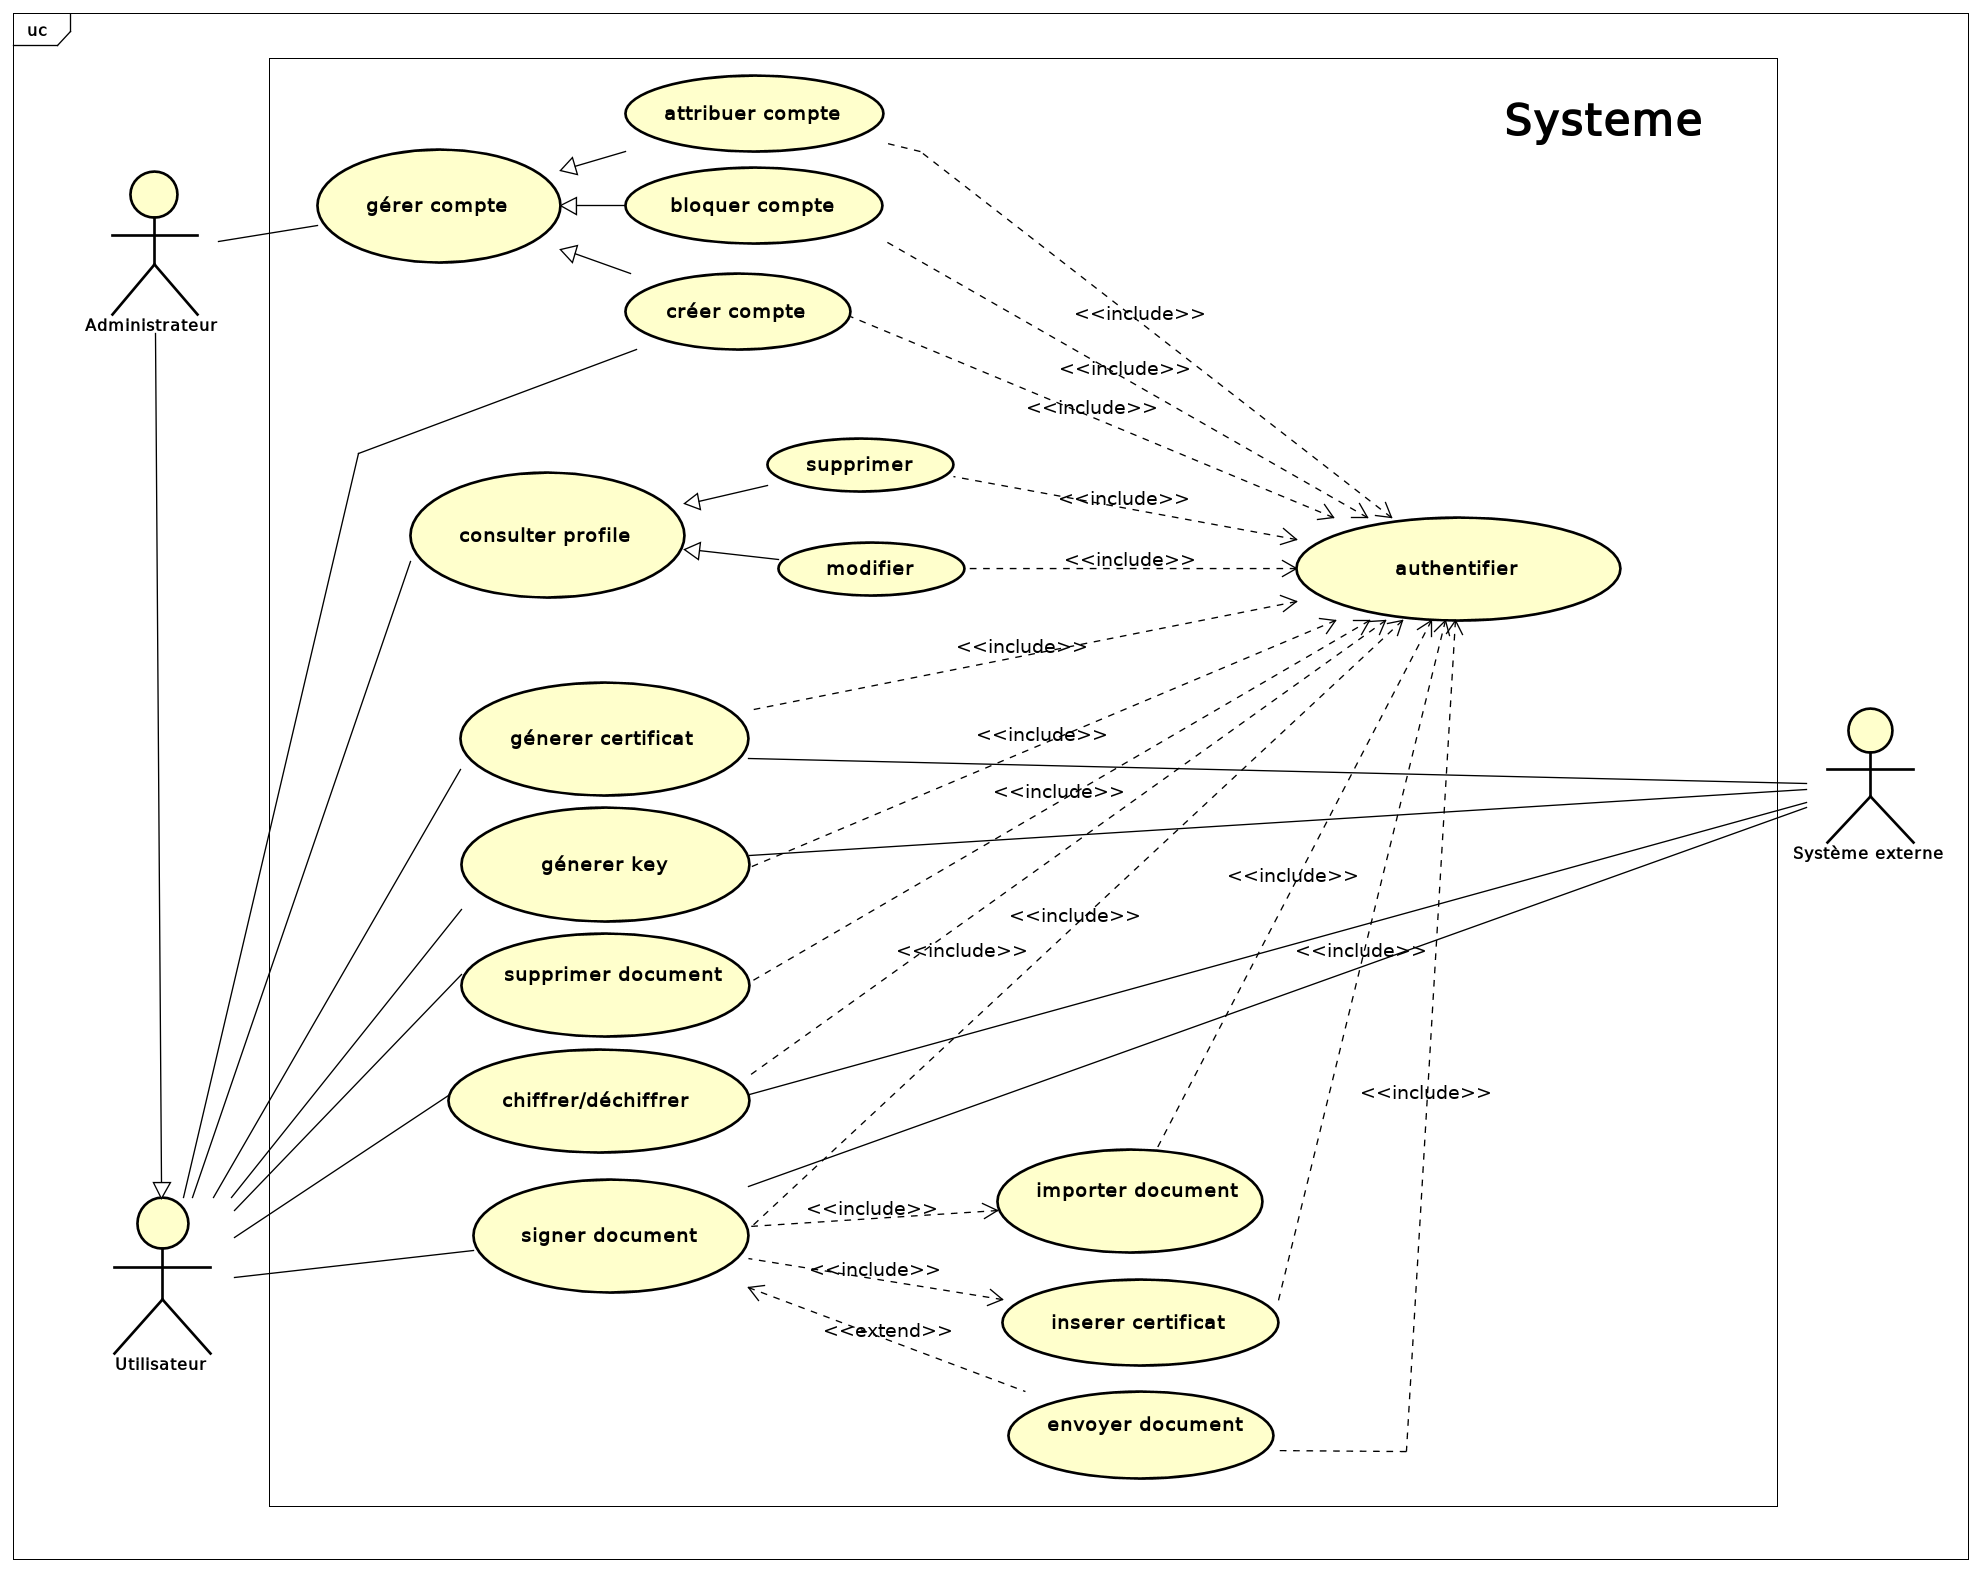
\includegraphics[width=18cm, height=9cm]{../Diagrammes/DiagrammeDeCasDutilisation/diagrammeGeneral.png} 
					\caption{Diagramme de cas d'utilisation général}
					\label{fig2}
			\end{figure}
			
		\textbf{Diagramme de cas d'utilisation de l'Administrateur :}
			\begin{figure}[H]
					\centering		
					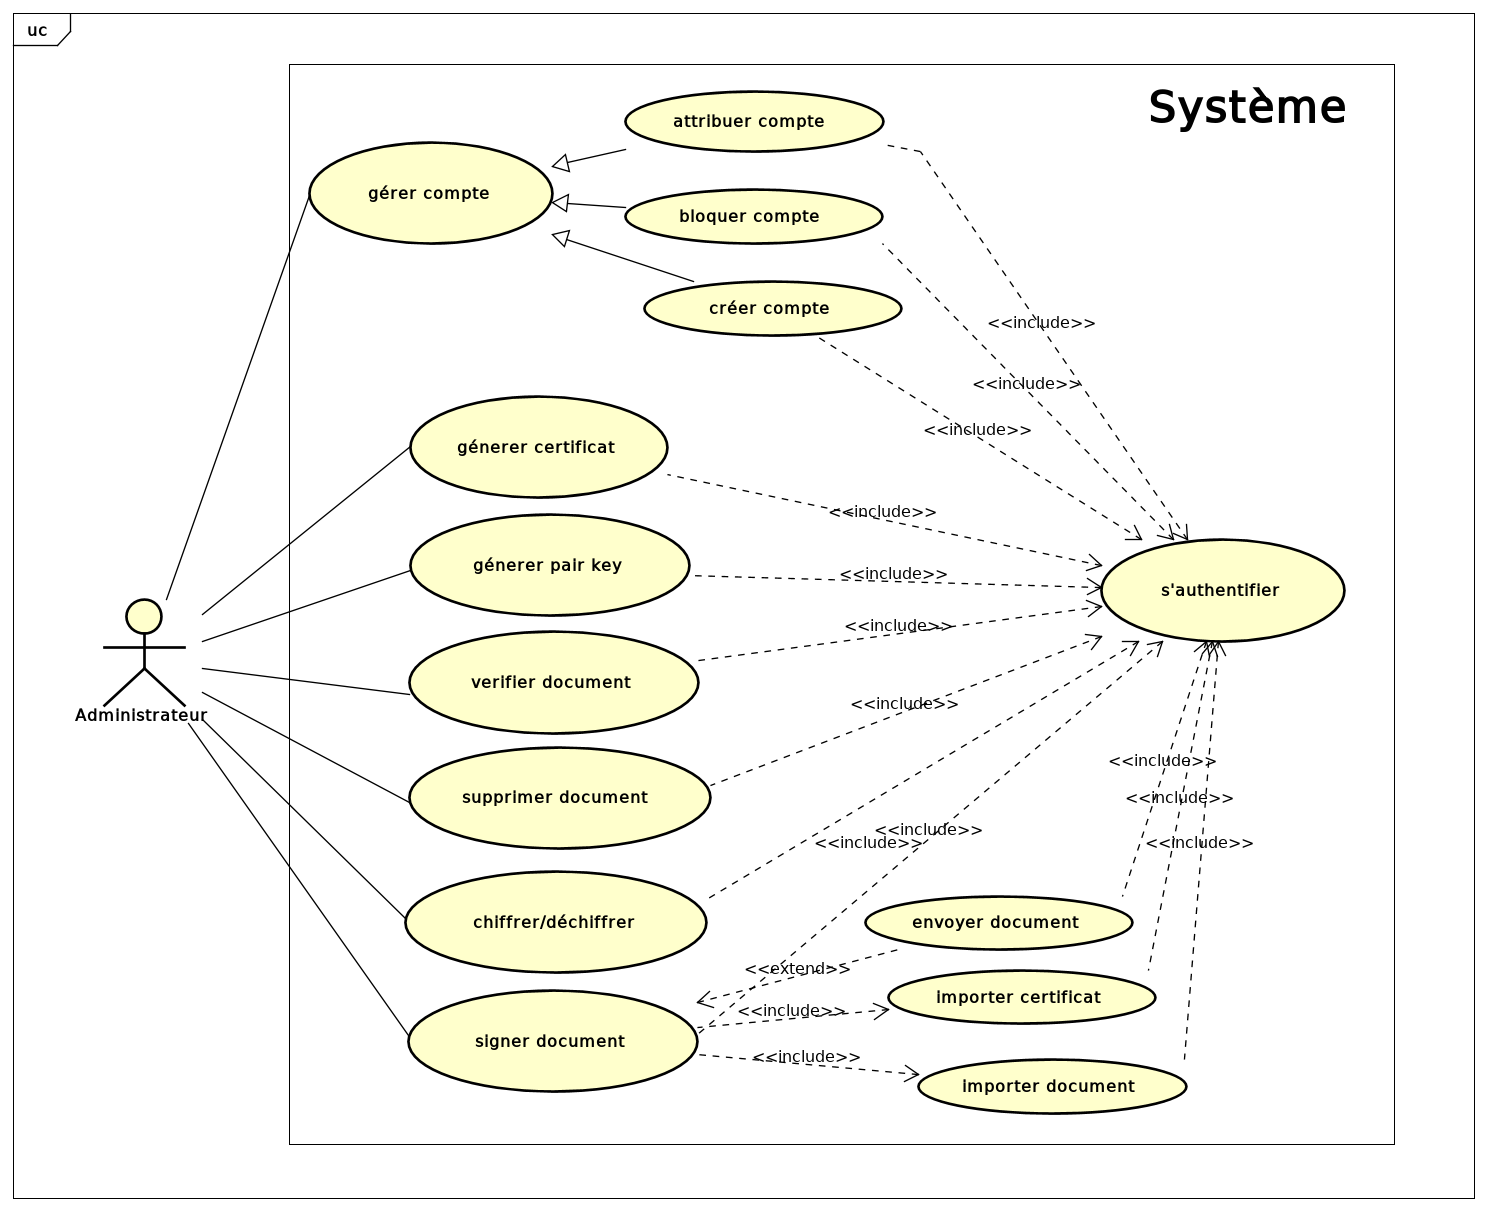
\includegraphics[width=18cm, height=8cm]{../Diagrammes/DiagrammeDeCasDutilisation/admin.png}  
					\caption{Diagramme de cas d'utilisation d'administrateur}
					\label{fig3}
			\end{figure}
		
		\textbf{Diagramme de cas d'utilisation de l'utilisateur :}
			\begin{figure}[H]
					\centering		
					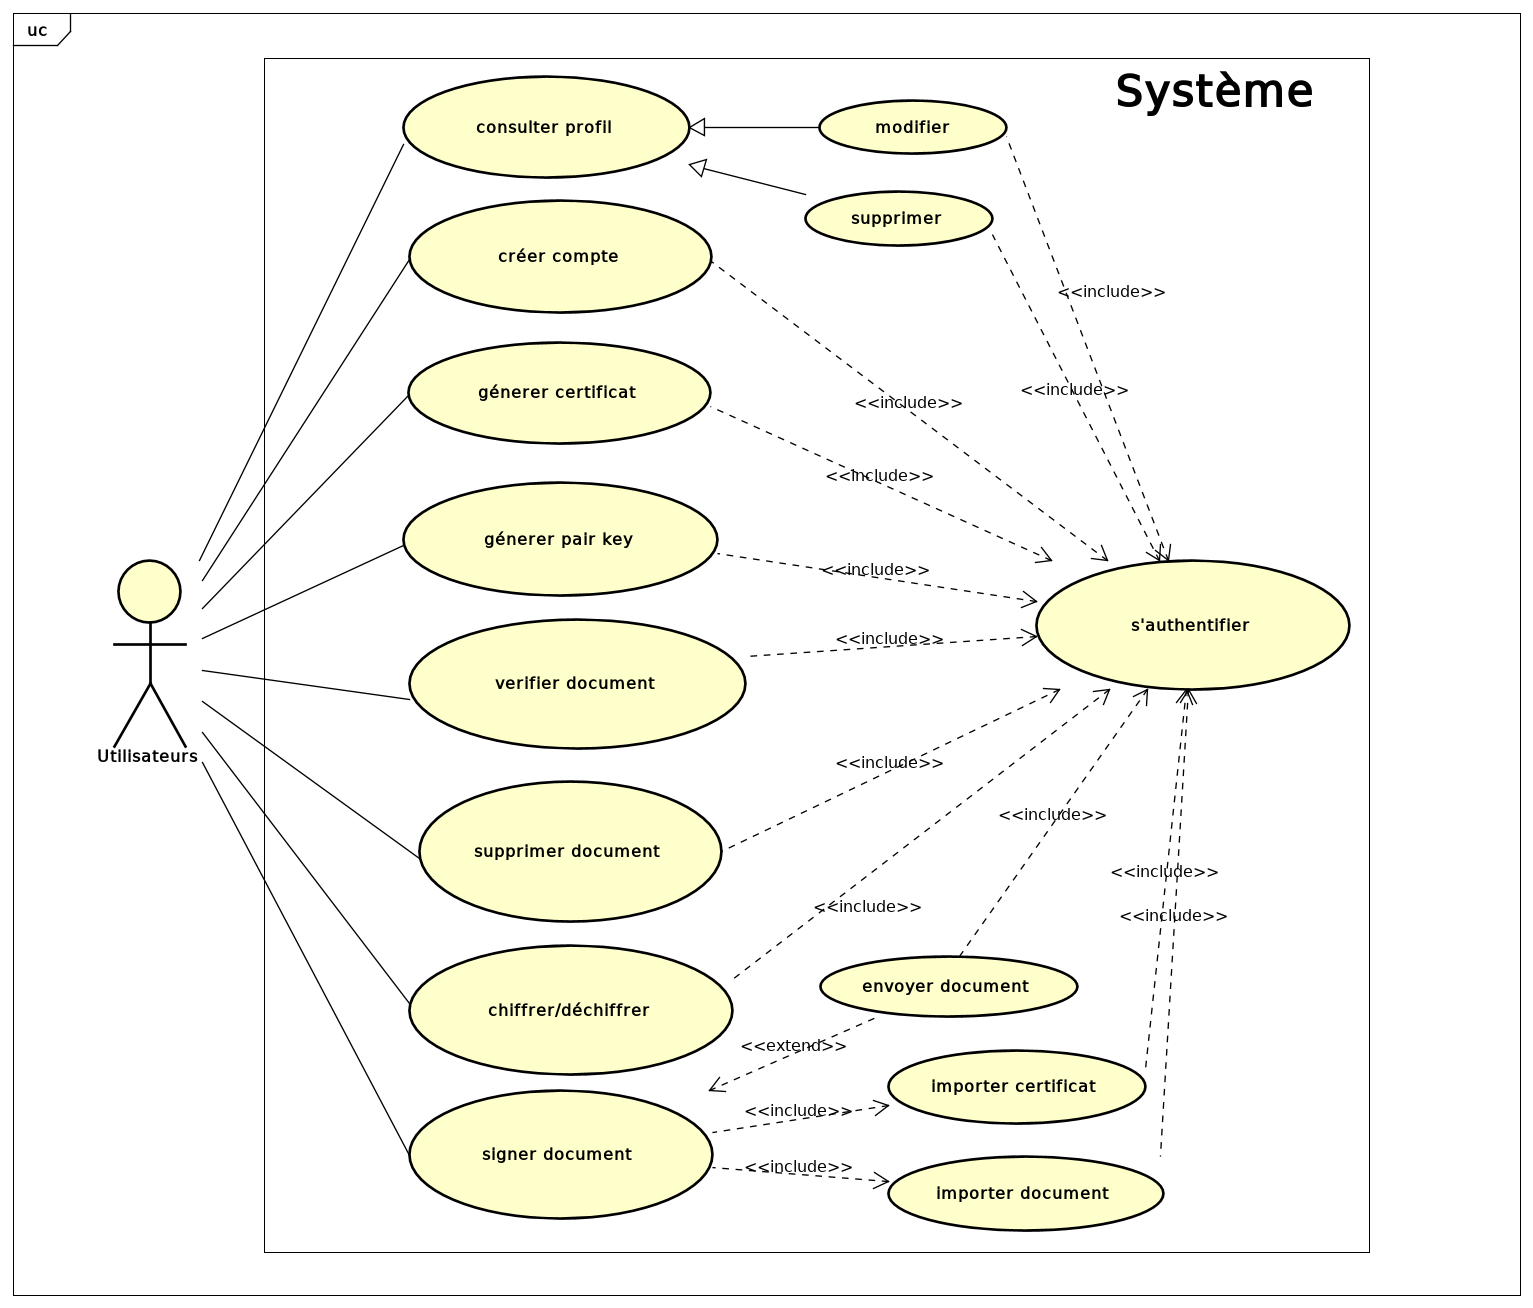
\includegraphics[width=18cm, height=8cm]{../Diagrammes/DiagrammeDeCasDutilisation/users.png}  
					\caption{Diagramme de cas d'utilisation d'utilisateur}
					\label{fig4}
			\end{figure}
			
			
	
			\textbf{Diagramme de cas d'utilisation de système externe :}
			\begin{figure}[H]
					\centering		
					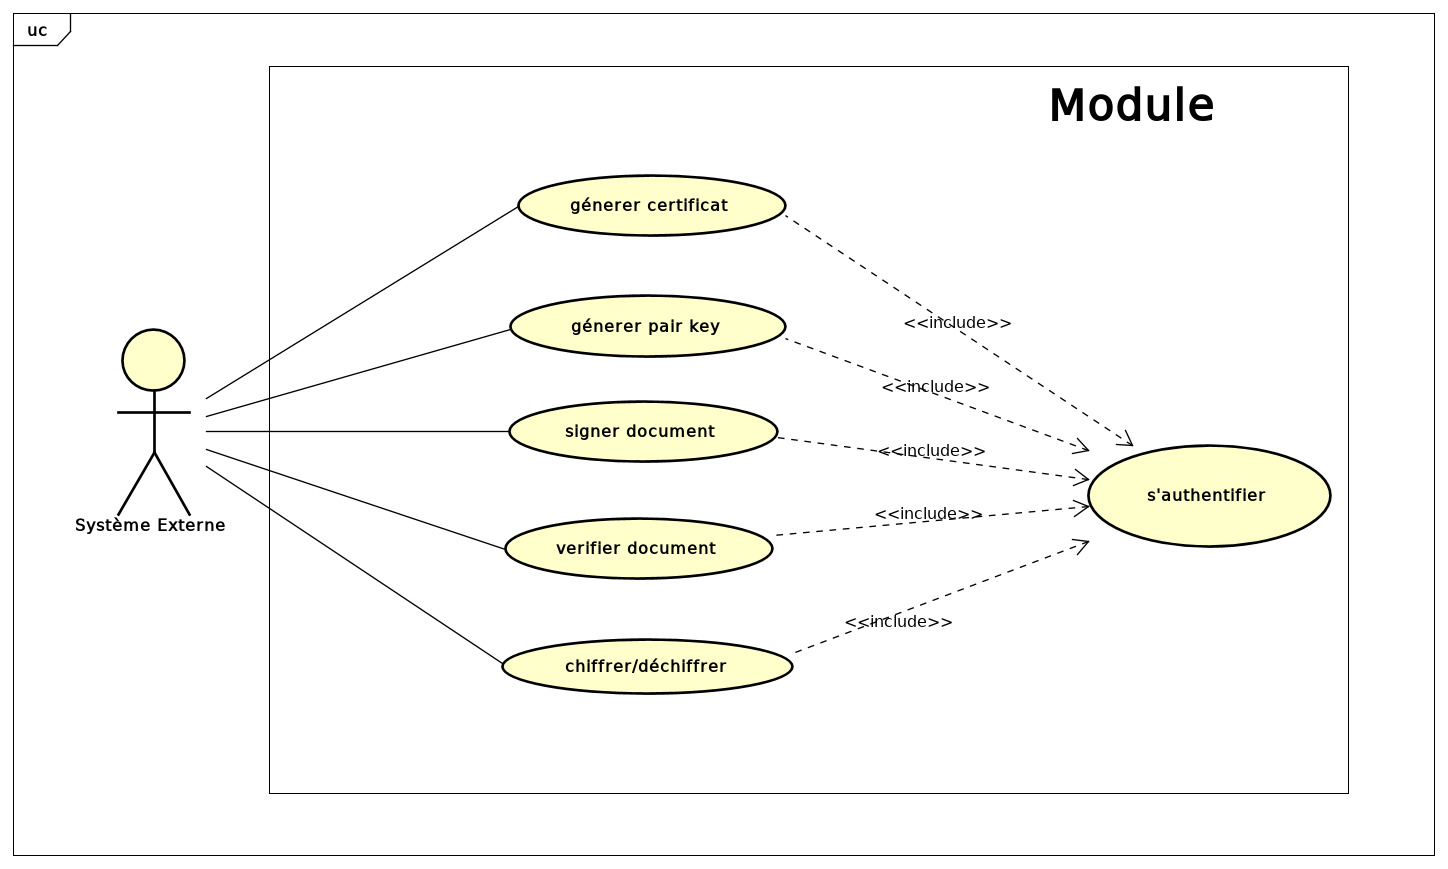
\includegraphics[width=18cm, height=8cm]{../Diagrammes/DiagrammeDeCasDutilisation/systemeexterne.png}  
					\caption{Diagramme de cas d'utilisation de système externe}
					\label{fig5}
			\end{figure}
			
	
			\subsubsection{Description textuelle de cas d'utilisation : S'authentifier}
			
			\begin{table}[H]
			
				\centering
					\caption{Description contextuelle de cas d'utilisation s'authentifier}
				\begin{tabular}{|l|p{11cm}|}
					\hline 
						\textbf{Titre} & S'authentifier \\ 
					\hline 
						\textbf{Résumé} & Ce cas d'utilisation permet d'accéder au tableau de bord de l'utilisateur \\ 
					\hline 
						\textbf{Acteur} & Administrateur, utilisateur \\  
				
					\hline 
						\textbf{Pré-condition} & l'application doit être lancer(page d'accueil) \\ 
					\hline 
						\multirow{2}{*}{\textbf{Scenario nominal}} & 1) l'utilisateur fait une demande l'accès au système en cliquant sur le bouton connexion, \\
							 & 2) le système lui renvoi le formulaire de connexion \\
							 & 3) l'utilisateur introduit son username et password \\
							 & 4) le système vérifie que  sont username et password corrects \\
							 & 5) le système ouvre une session de l'utilisateur \\
					\hline 
					
						\multirow{2}{*}{\textbf{Enchaînement Alternatif}} & le username et le password sont corrects., \\
							  & l'enchaînement commence au point 3 du scénario nominal. \\
							 & le message affiche un message d'erreur, aller au point 2. \\
					\hline 
						\textbf{Enchaînement d'Erreur} & E1 : Si l'étape 2 de scenario nominal n'est pas vérifié un message d'erreur sera affiché. \\
					\hline
						\textbf{Post condition} & ouverture d'une session, accès au compte\\
					\hline
				
			\end{tabular} 
			
		\end{table}
		
		
		
		\subsubsection{Description textuelle de cas d'utilisation : Générer certificat}
		
			\begin{table}[H]
			
				\centering
					\caption{Description contextuelle de cas d'utilisation générer certificat}
				\begin{tabular}{|l|p{11cm}|}
					\hline 
						\textbf{Titre} & Générer Certificat \\ 
					\hline 
						\textbf{Résumé} & Ce cas d'utilisation permet de générer des certificats aux utilisateurs \\ 
					\hline 
						\textbf{Acteur} & Autorité de certification Administrateur, Système externe \\  
				
					\hline 
						\textbf{Pré-condition} & l'application doit être lancer (page d'accueil) \\ 
					\hline 
						\multirow{2}{*}{\textbf{Scenario nominal}} & 1) un AC peut générer un certificat en cliquant sur le bouton genererCertifcat, \\
							 & 2) le système lui renvoi le formulaire à remplir \\
							 & 3) on introduit la clé publique de l'utilisateur \\
							 & 4) on renseigne le nom et le prénom de l'utilisateur \\
							 & 5) la date de validité (début et fin)\\
							 & 6) numéro de version\\
							 &7) numéro de série. \\
					\hline 
					
						\multirow{2}{*}{\textbf{Enchaînement Alternatif}} & la clé publique n'est pas corrects. \\
							  & l'enchaînement commence au point 2 du scénario nominal. \\
							
					\hline 
						\textbf{Enchaînement d'Erreur} & E1 : Si l'étape 2 de scenario nominal n'est pas vérifié un message d'erreur sera affiché. \\
					\hline
						\textbf{Post condition} & création de certificat avec succès.\\
					\hline
				
			\end{tabular} 
			
		\end{table}
	
		
	\subsubsection{Description textuelle de cas d'utilisation : Générer Paire de Clé}
	
				\begin{table}[H]
			
				\centering
					\caption{Description contextuelle de cas d'utilisation générer paire de clé}
				\begin{tabular}{|l|p{11cm}|}
					\hline 
						\textbf{Titre} & Générer Paire de clé \\ 
					\hline 
						\textbf{Résumé} & Ce cas d'utilisation permet de générer des paires de clé aux utilisateurs \\ 
					\hline 
						\textbf{Acteur} & Autorité de certification, Administrateur, Système externe, Utilisateur \\  
					\hline 
						\textbf{Pré-condition} & l'application doit être lancer (page d'accueil) et l'utilisateur est authentifié \\ 
					\hline 
						\multirow{2}{*}{\textbf{Scenario nominal}} & 1) un utilisateur peut générer une paire en cliquant sur le bouton genererPaireKey, \\
							 & 2) le système lui renvoi le formulaire à remplir \\
							 & 3) il introduit le cryptosystème à utiliser (ex. RSA) \\
							 & 4) ensuite il introduit la taille de clé (ex.4096) \\
							 & 5) il valide en cliquant sur le bouton générer \\
					\hline 
					
						\multirow{2}{*}{\textbf{Enchaînement Alternatif}} & l'algorithme ou la taille de clé est incorrect. \\
							  & l'enchaînement commence au point 2 du scénario nominal. \\
							
					\hline 
						\textbf{Enchaînement d'Erreur} & E1 : Si l'étape 3 de scenario nominal est incorrect, un message d'erreur sera affiché. \\
						& Si l'étape 4 de scenario nominal est incorrect, un message d'erreur sera affiché. \\
					\hline
						\textbf{Post condition} & génération de paire de clé avec succès.\\
					\hline
				
			\end{tabular} 
			
		\end{table}
		
	\subsubsection{Description textuelle de cas d'utilisation : Signer document}

				\begin{table}[H]
			
				\centering
					\caption{Description contextuelle de cas d'utilisation Signer document}
				\begin{tabular}{|l|p{11cm}|}
					\hline 
						\textbf{Titre} & Signer document \\ 
					\hline 
						\textbf{Résumé} & Ce cas d'utilisation permet aux utilisateurs de signer leurs documents \\ 
					\hline 
						\textbf{Acteur} & Autorité de certification, Administrateur, Système externe, Utilisateur \\ 
					\hline 
						\textbf{Pré-condition} & l'application doit être lancer (page d'accueil) et l'utilisateur est authentifié \\ 
					\hline 
						\multirow{2}{*}{\textbf{Scenario nominal}} & 1) un utilisateur peut signer son document en cliquant simplément sur le bouton Signer document, \\
							 & 2) le système lui renvoi le formulaire à remplir \\
							 & 3) il téléverse son fichier(txt, docs, pdf,etc) \\
							 & 4) ensuite il téléverse sa clé publique\\
							 & 5) il sélectionne la fonction de hachage (ex. SHA1, SHA256 ...)\\
							 & 6) il valide en cliquant sur le bouton Signer document \\
					\hline 
					
						\multirow{2}{*}{\textbf{Enchaînement Alternatif}} & l'algorithme est incorrect. \\
							  & l'enchaînement commence au point 2 du scénario nominal. \\
							
					\hline 
						\textbf{Enchaînement d'Erreur} & E1 : Si l'étape 3 de scenario nominal est incorrect, un message d'erreur sera affiché. \\
						& Si l'étape 4 de scenario nominal est incorrect, un message d'erreur sera affiché. \\
					\hline
						\textbf{Post condition} & La signature est effectuée avec succès.\\
					\hline
			\end{tabular} 
		\end{table}
	
	\subsubsection{Description textuelle de cas d'utilisation : Créer Compte}

			\begin{table}[H]
				\centering
					\caption{Description contextuelle de cas d'utilisation Créer Compte}
				\begin{tabular}{|l|p{11cm}|}
					\hline 
						\textbf{Titre} & Créer Compte \\ 
					\hline 
						\textbf{Résumé} & Ce cas d'utilisation permet aux utilisateurs de crées leurs comptent \\ 
					\hline 
						\textbf{Acteur} & Administrateur, Utilisateur \\ 
			
					\hline 
						\textbf{Pré-condition} & l'application doit être lancer (page d'accueil)  \\ 
					\hline 
						\multirow{2}{*}{\textbf{Scenario nominal}} & 1) l'utilisateur peut créer un compte en cliquant sur le bouton \textbf{créer un compte} \\
							 & 2) le système lui renvoi le formulaire à remplir \\
							 & 3) il entre son nom, prénom, mot de passe, E-mail \\
							 & 4) et il valide en cliquant sur le bouton créer\\
					\hline 
					
						\multirow{2}{*}{\textbf{Enchaînement Alternatif}} & l'adresse E-mail est incorrect. \\
							  & l'enchaînement commence au point 2 du scénario nominal. \\
							
					\hline 
						\textbf{Enchaînement d'Erreur} & E1 : Si l'étape 3 de scenario nominal est incorrect, un message d'erreur sera affiché. \\
					\hline
						\textbf{Post condition} & Le compte est crée avec succès.\\
					\hline	
			\end{tabular} 
		\end{table}
	
	
	\subsubsection{Description textuelle de cas d'utilisation : Envoyer Document}

				\begin{table}[H]
				\centering
					\caption{Description contextuelle de cas d'utilisation Envoyer Document}
				\begin{tabular}{|l|p{11cm}|}
					\hline 
						\textbf{Titre} & Envoyer Document \\ 
					\hline 
						\textbf{Résumé} & Ce cas d'utilisation permet aux utilisateurs d'envoyer leurs document signer \\ 
					\hline 
						\textbf{Acteur} & Administrateur, Utilisateur \\ 
			
					\hline 
						\textbf{Pré-condition} & l'application doit être lancer (page d'accueil) et l'utilisateur est authentifié  \\ 
					\hline 
						\multirow{2}{*}{\textbf{Scenario nominal}} & 1) un utilisateur peut envoyer un document en cliquant sur l'onglet message \textbf{Envoyer document} \\
							 & 2) le système lui renvoi le formulaire à remplir \\
							 & 3) il téléverse son document \\
							 & 4) il téléverse son certificat\\
							 & 5) ensuite il choisit un destinateur\\
							 & 6) enfin il valide en cliquant sur le bouton \textbf{Envoyer}.\\
					\hline 
					
						\multirow{2}{*}{\textbf{Enchaînement Alternatif}} & l'adresse E-mail est incorrect. \\
							  & l'enchaînement commence au point 2 du scénario nominal. \\
							
					\hline 
						\textbf{Enchaînement d'Erreur} & E1 : Si l'étape 5 de scenario nominal est incorrect, un message d'erreur sera affiché. \\
					\hline
						\textbf{Post condition} & L'envoi est effectué avec succès.\\
					\hline
			\end{tabular} 
		\end{table} 
	
		
	
	
	
	
	
	
	
	 
	
	
	
	
	
	

%\end{flushleft}
\end{document}